\subsection{Heart Modeling}
 \label{sec:heart modeling}
The heart model has two components: a timing model and a morphology model.

\subsubsection{Timing Model}
\begin{figure}[t]
	\centering
	\vspace{-10pt}
	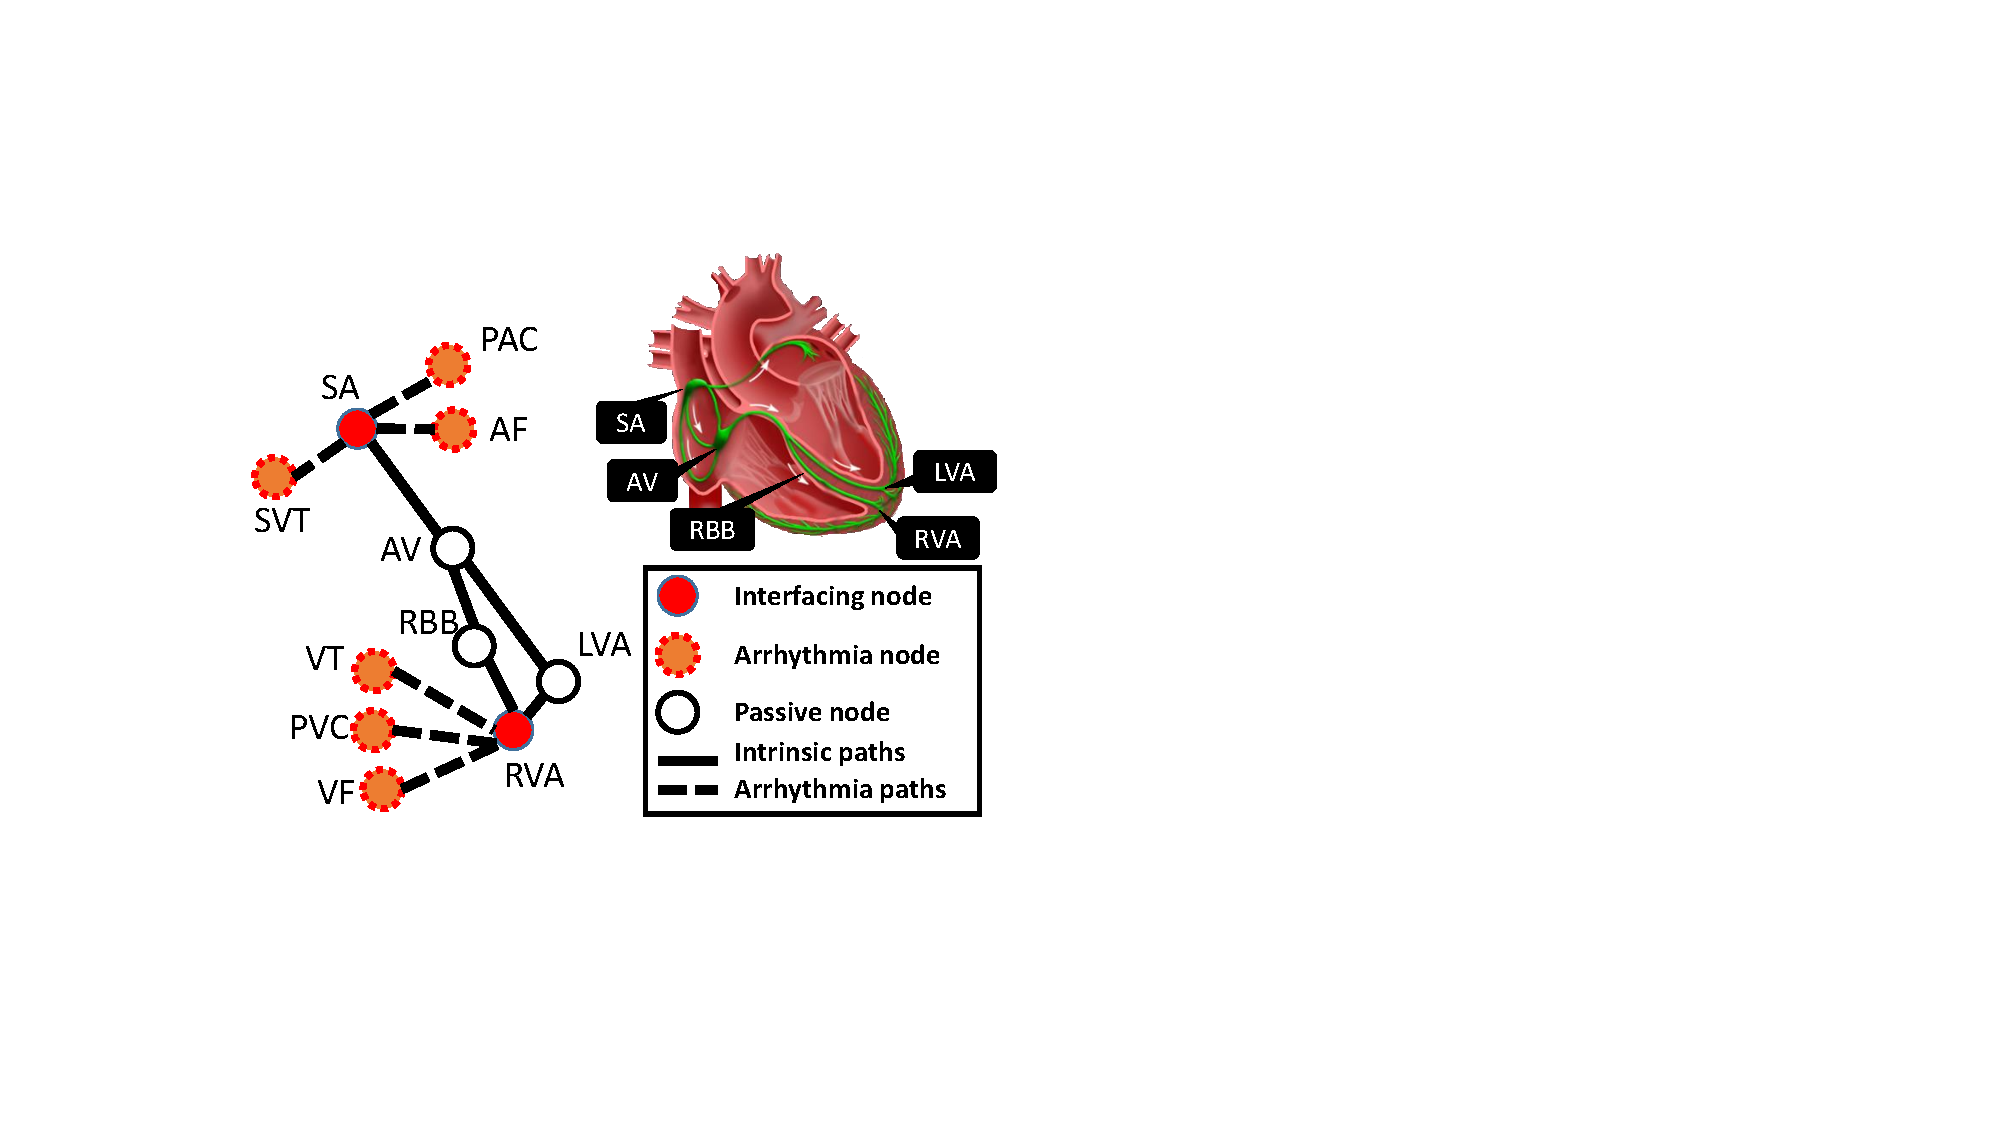
\includegraphics[width=0.3\textwidth]{figures/HM_top.pdf}
	\caption{\small Timing model of the heart}
	\vspace{-10pt}
	\label{fig:HM_top}
\end{figure}

Because the relative timing of atrial and ventricular events is an essential part of an arrhythmia's clinical definition, it is important that our model capture correctly the broad range of timings of various arrhythmias.
To this end, we developed an automaton model of the heart that simulates event sequences in atrium and ventricle shown in Fig. \ref{fig:HM_top}. 
Each filled node represents a potential source of spontaneous electrical activity, i.e., a potential source of an event.
For example, the SA node is the source of \ac{NSR}.
The \emph{dashed} filled nodes represent sources of \emph{abnormal} rhythms: e.g., the PAC node can produce Premature Atrial Complexes (a.k.a. ectopics), and the VF node can produce a ventricular fibrillation rhythm.

The hollow nodes (AV, RBBB, LVA) do not produce events. 
Rather, they are passive nodes representing key locations within the heart where electrical propagation may be blocked or delayed.
The paths connecting nodes represent bi-directional paths of propagation of electrical activity in the heart.
Thus an SA event propagates down to the RVA node via paths and the AV node, while a VF rhythm can propagate back to the atria via the LVA and AV nodes.

Each node and path has a set of timing parameters that control the rate, the delay between events, the conduction delay in a path, and how the rhythm changes from beat to beat, e.g., as a result of the refractory period.
By varying these parameters, we can simulate the timing of a wide variety of arrhythmias, and even vary the timing of a given arrhythmia beat-to-beat.
These timing parameters can be directly derived from clinical data \cite{josephson}, thus we know the ranges for these parameters.
In \cite{VHM_proc}, the timing model's capability to simulate various normal and abnormal heart conditions was validated quantitatively and by cardiac electrophysiologists. 
See Fig.~\ref{fig:mbct overview} \circled{2}.

\subsubsection{Morphology Model}
\emph{For a given patient}, it has been clinically observed that \ac{EGM} signals from the same source (i.e. the same location in the heart) generally have the same morphology. 
In our timing model, we have 5 different sources for SA node activation (the 5 dashed nodes connected to the SA node) and 5 different sources for RVA node activation (5 dashed nodes connected to the RVA node). 
Assume that we have a database of \acp{EGM}, where each \ac{EGM} has the distinctive morphology of that source, and is labeled with that source.
E.g., we have \acp{EGM} labeled `SA', others labeled `VF', etc.
(In next section, we explain how to build this database from real patients' data).
Given a sequence of atrial and ventricular events generated by the timing model, each event simply gets an \ac{EGM} that is labeled with that event's source (Fig. \ref{fig:egmGeneration}).
Concatenated, these give an entire arrhythmia episode.
To avoid repeating the exact same \ac{EGM}, which is unrealistic, we also introduce small variations on EGM templates.
The variations are obtained by a wavelet decomposition of the signatures followed by a random scaling of the 25\% smallest coefficients.
We guarantee that this does not change the labeling of the \ac{EGM} by running one of the morphology comparison discriminators used in the ICD.
See Fig.~\ref{fig:mbct overview} \circled{1}.

\begin{figure}[t]
	\centering
	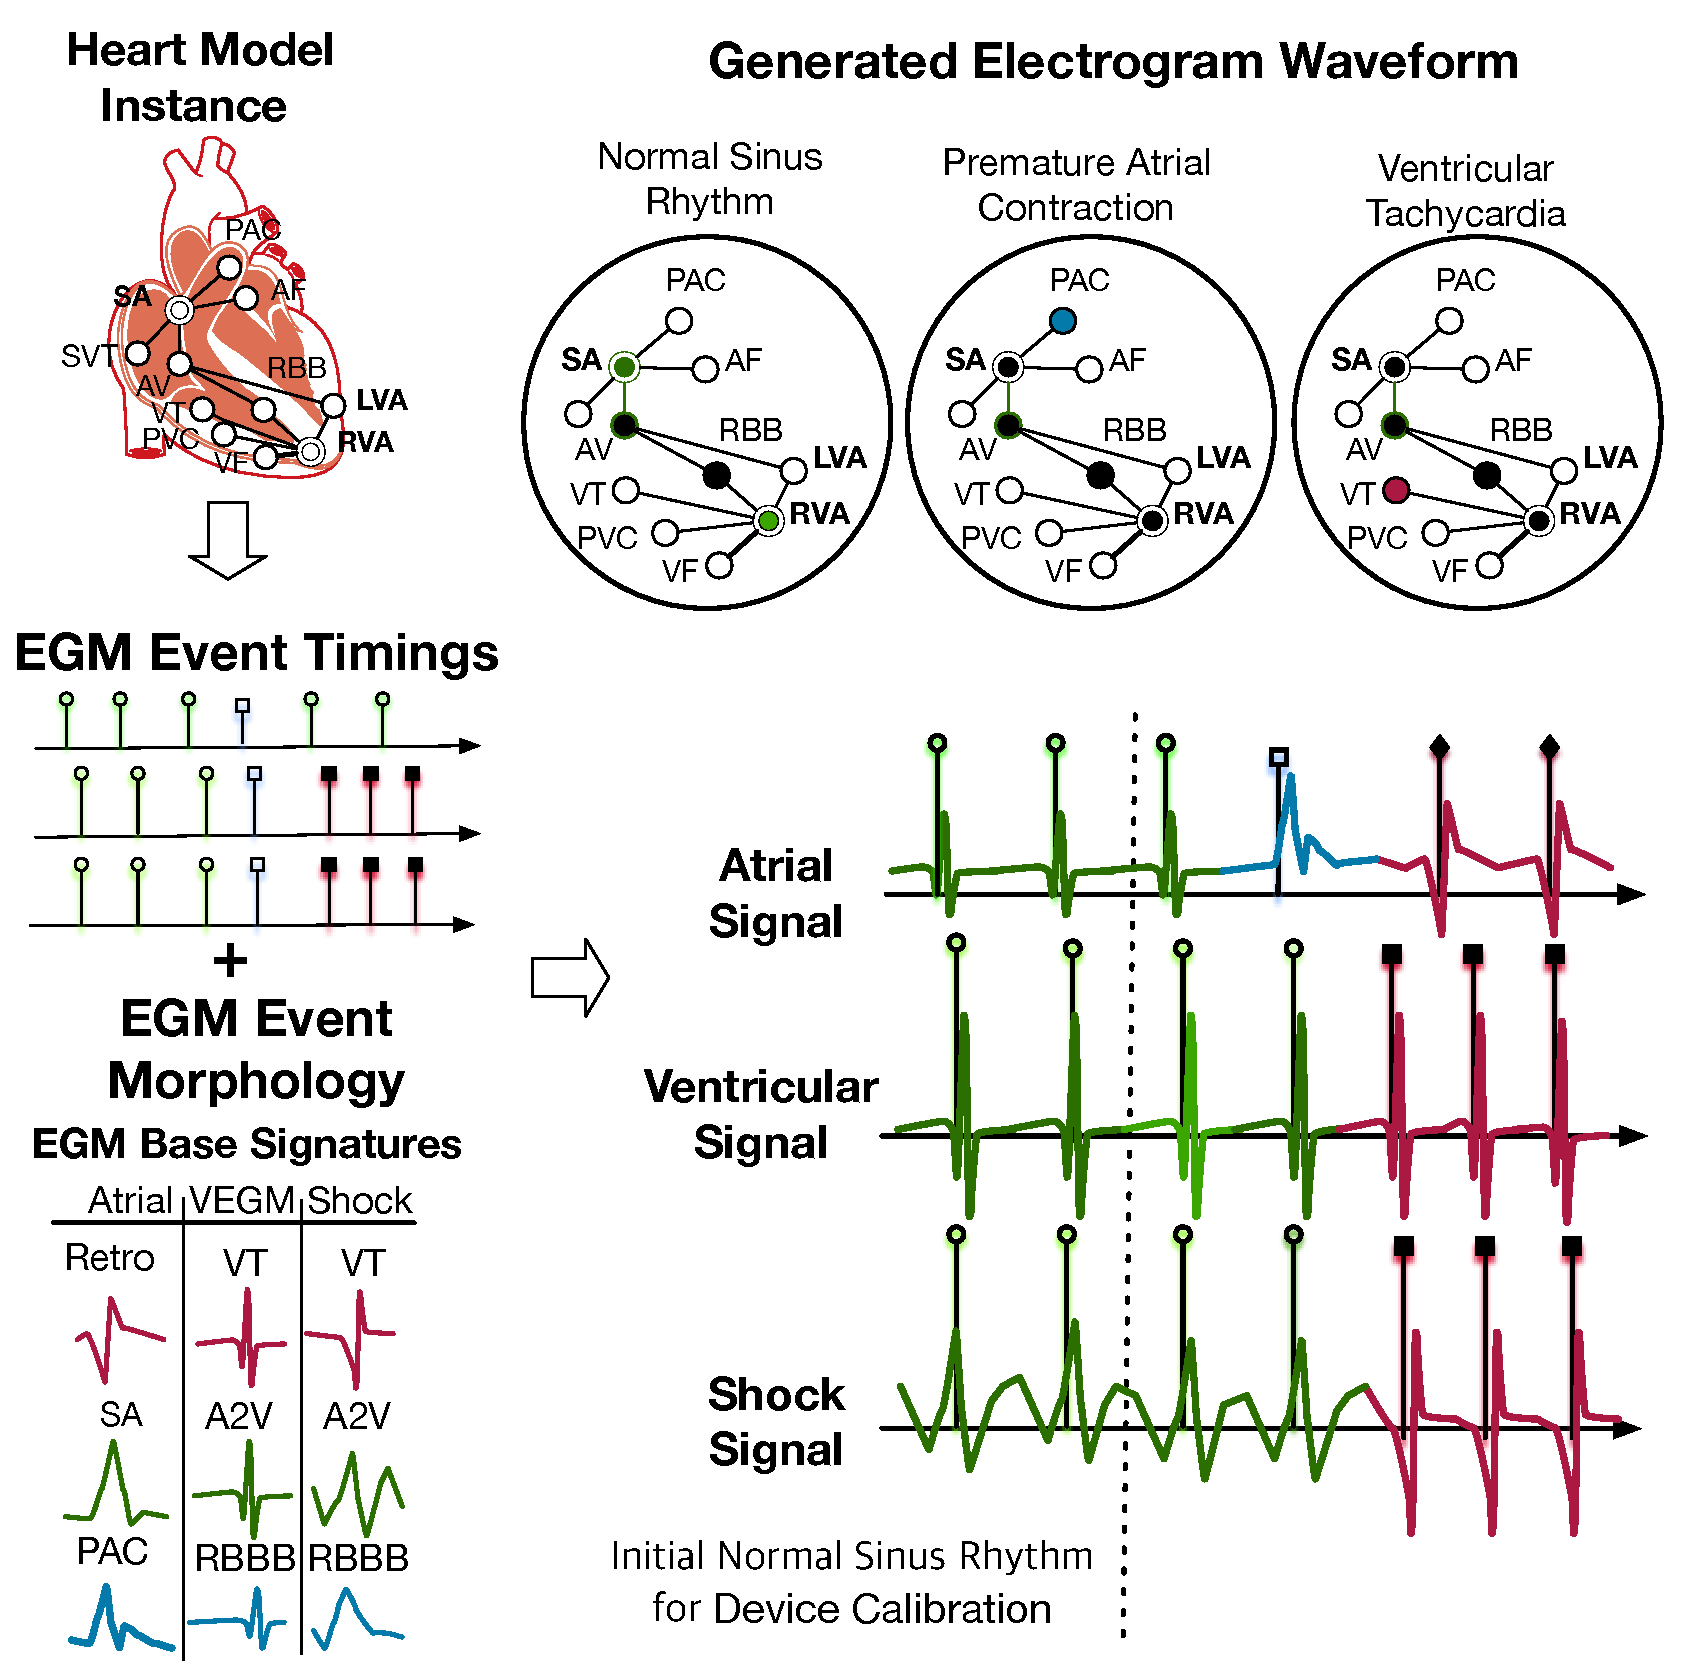
\includegraphics[scale=0.3]{figures/figEGMGeneration1column.pdf}
	\vspace{-15pt}
	\caption{\small \ac{EGM} waveform generation.
		From a given model instance and set of tachycardias, an EGM waveform is generated for the duration of an episode. The timing model determines event timings. When an event occurs, the EGM morphology for the event is output from the morphology model.  
		}
	\vspace{-15pt}
	\label{fig:egmGeneration}
\end{figure}

 \subsection{Patient Data Adjudication and EGM Template Extraction}
In order to obtain realistic morphologies for our simulations we utilize the Ann Arbor Electrogram Libraries (AAEL), a database of over 500 \ac{EGM} recordings made during clinical electrophysiology studies~\cite{AAEL}. 
The AAEL is used by all major \ac{ICD} manufacturers and is licensed by the US FDA. 
The AAEL provides descriptive annotations of records at a high level.
We performed additional detailed examination to precisely segment each record according to rhythm type.
123 records from 47 patients were manually examined and adjudicated into segments called \emph{episodes} containing one specific rhythm, e.g.\, \ac{NSR} or \ac{VF}. 
The adjudication was performed by a cardiologist.
Fig. \ref{fig:adjudication} (left) shows an example record (Record A185660) which has undergone this adjudication.
%It should be noted that only with a standard 12-lead \ac{ECG} in addition to ICD signals can all types of arrhythmia be accurately diagnosed.
From each episode, we developed an automated process which extracted \ac{EGM}s from a given episode. 
The \ac{EGM} are collected and organized by both patient record and by the type of rhythm which was annotated during the adjudication process.
These extracted rhythm \emph{signatures} provide the basis for the morphology information in the signal generated by our model.
Fig. \ref{fig:adjudication} (right) depicts an example of 10 signatures extracted from the record. 

\begin{figure*}[t]
	\centering
	\vspace{-10pt}
	\includegraphics[scale=0.35]{figures/figadjudication.pdf}
	\vspace{-10pt}
	\caption{\small  (Left) The \ac{EGM} record is segmented into episodes with distinct rhythms in each. (Right) From each episode, individual \acp{EGM} morphologies are extracted and stored.
	}
	\label{fig:adjudication}
\end{figure*}
%(Left) Adjudication of record A185660 
%(right) Examples of \ac{EGM} morphology signatures extracted from record: SA - Sinoatrial Node Event; Retrograde - Atrial event from Ventricular Retrograde; A2V - Sinus Atrial to Ventricular Conduction; A2V Shock - Shock signal of Sinus Atrial to Ventricular Conduction; PVC - Premature Ventricular Contraction Event; PVC Shock - Shock signal of Premature Ventricular Contraction Event; VT - \ac{VT} event; VT Shock - Shock signal of \ac{VT} event;  VF - \ac{VF} event; VF Shock - Shock signal of \ac{VF} event
%Our starting point is the AAEL database of \ac{EGM}s \cite{AAEL}.
%These are \ac{EGM} records collected from real patients during electrophysiologic testing.
%We worked with 123 records from 47 patients (a patient may have more than one recording session).
%We segmented each record into \emph{episodes}: an episode is a segment of a record with one main rhythm, e.g., Normal Sinus Rhythm or Ventricular Fibrillation.
%For a given rhythm, the database generally contains several episodes.
%Then from each episode of each rhythm, we extracted a number of electrograms, say, 10.
%The extracted \ac{EGM}s provide a \emph{signature} for what the \ac{EGM} looks like during that particular rhythm.
%Fig. \ref{fig:adjudication} illustrates the process of obtaining these signatures, as well as the extracted \ac{EGM}s and the rhythms of the episodes from which they were extracted.\begin{figure*}[t]
%		\centering
%		\includegraphics[scale=0.4]{figures/figadjudication.pdf}
%		\caption{\small Examples of \ac{EGM} morphology with different signatures.
%			 }
%		\label{fig:adjudication}
%\end{figure*}

\subsubsection{Cohort generation}
\label{sec:cohort generation}
See Fig.~\ref{fig:mbct overview}.
Let $p = (p_1,\ldots,p_n) \in \Re^n$ be the vector of parameters of the heart model.
Let $P_i \subset \Re$ be the range of parameter $p_i$.
We generate a \emph{synthetic cohort} of $N$ probabilistic model instances.
To produce one of these instances, for each scalar parameter $p_i$, we randomly select a sub-interval $I_i$ of its range: $I_i \subset P_i$.
The sub-interval $I_i$ is chosen so that it fits with the tachycardia that this model instance is meant to simulate.
E.g., for modeling \ac{VT}, the rest period of the \ac{VT} node might be assigned the sub-interval $I_i = [260, 280]ms$, reflecting the firing rate in the ventricles.
%Two different instances of the same tachycardia will, in general, have different sub-intervals within $P_i$.
When a model instance is simulated, each parameter $p_i$'s value changes beat to beat by sampling it uniformly within its sub-interval $I_i$.
Thus each generated model is probabilistic to reflect inherent rhythm variability.